\newpage
\part{Makromolekyler}
    \section*{Redegør for opbygning af de makromolekyler der findes i fødevarer.}
        Der er 4 forskellige makromolekyler i fødevarer, nemlig kulhydrater, proteiner, fedtstoffer, og nukleinsyrer. Jeg vil mest komme ind på de 3 første. 
        \subsection**{Lipider (fedtstoffer)}
           Den normale måde at indtage fedt på er ved triglycerid. Fedt er vigigt for kroppen da det er en energi kilde. Fedt er også vigtigt for kroppen da det er med til at danne cellemembranen. Fedt er også med til at danne hormoner.
           Lipider er en bred klasse af biologiske molekyler, der er kendetegnet ved deres opløselighed i ikke-polar organiske opløsningsmidler og deres uopløselighed i vand. Lipider kan opdeles i forskellige undergrupper baseret på deres struktur, herunder triglycerider, fosfolipider, steroler og andre. Her er en kort beskrivelse af strukturen af nogle af de mest almindelige typer lipider:

           \textbf{Triglycerider:} Dette er den mest almindelige type lipid og den form, hvori kroppen opbevarer fedt. En triglycerid består af et glycerolmolekyle, der er bundet til tre fedtsyremolekyler. Fedtsyrer er lange kæder af carbon og hydrogen, der kan variere i længde. Fedtsyrerne kan være mættede (ingen dobbeltbindinger mellem carbonatomer) eller umættede (en eller flere dobbeltbindinger). Når vi taler om fedtsyrer, snakker man om "mættet" og "umættet" til strukturen af fedtsyrekæden, især til antallet af dobbeltbindinger mellem carbonatomerne i kæden.
           Mættede fedtsyrer: Mættede fedtsyrer har ingen dobbeltbindinger mellem carbonatomerne. Dette betyder, at hvert carbonatom er bundet til (eller "mættet med") det maksimale antal hydrogenatomer. Mættede fedtsyrer er typisk faste ved stuetemperatur og findes i animalske produkter som kød og mejeriprodukter, samt i nogle plantefødevarer som kokos- og palmeolie.
           
           Umættede fedtsyrer: Umættede fedtsyrer har en eller flere dobbeltbindinger mellem carbonatomerne. Dette betyder, at kæden ikke indeholder det maksimale antal hydrogenatomer - den er "umættet". Dobbeltbindingerne forårsager en knæk eller bøjning i fedtsyrekæden. Umættede fedtsyrer er typisk flydende ved stuetemperatur og findes i fødevarer som fiskeolie, olivenolie, rapsolie og nødder.
           
           Umættede fedtsyrer kan yderligere kategoriseres som "enkeltumættede" (hvis de har en dobbeltbinding) eller "flerumættede" (hvis de har mere end en dobbeltbinding). Omega-3 og omega-6 fedtsyrer, som du nævnte tidligere, er typer af flerumættede fedtsyrer.

            \textbf{Fosfolipider:} Fosfolipider er hovedkomponenten i cellemembraner. De har en struktur, der ligner triglycerider, men en af fedtsyrerne er erstattet med en fosfatgruppe. Dette gør en del af molekylet polært (og derfor vandopløseligt), mens resten af molekylet er nonpolært (og derfor uopløseligt i vand). Denne amfipatiske natur tillader fosfolipider at danne lipidbilag, som er grundlaget for cellemembraner.

            \textbf{Steroler:} \\ Steroler, som kolesterol, er en type lipid, der er kendetegnet ved en kompleks ringstruktur. Kolesterol er en vigtig komponent i cellemembraner, hvor det bidrager til fluiditet og stabilitet. Det er også forløberen for andre biologisk vigtige molekyler, herunder steroidhormoner, galdesalte og vitamin D.


            
        \subsection**{Kulhydrater - Sakarid}
        Mennesker har altid fået en stor del af deres energi i form af kulhydrater. Under fordøjelsen omdannes kulhydrater til glukose. Hjernens primære brændstof er glukose, og bl.a. derfor er kulhydrater en vigtig energikilde. I kulhydrater findes kulstof (C), brint (hydrogen (H)) og ilt (oxygen (O)) altid i forholdet 1:2:1. Derfor kan de almindeligste kulhydrater skrives efter Formlen: \begin{math}(CH_2O)_n\end{math}.
        Kulhydrater benævnes efter antallet af kulstofatomer i molekylet, hvorfor trioser, tetroser, pentoser og hexoser indeholder hhv. tre, fire, fem og seks kulstofatomer.
        Ernæringsmæssigt er det kun hexoserne, glukose og fruktose, der er interessante, fordi det er dem, der overvejende optages og omsættes i kroppen.
        Et kulhydratmolekyle kaldes et monosakkarid, når det ikke kan spaltes yderligere til et kulhydrat. Flere monosakkarider kan bindes til hinanden, hvorved der dannes kæder med eller uden forgrening. Disse kæder af monosakkarider inddeles efter, hvor mange monosakkarider som er bundet sammen. Således vil et disakkarid indeholde to monosakkarider, mens oligosakkarider og polysakkarider vil indeholde hhv. 3-9 og over 9 monosakkarider i molekylet. 
        \begin{figure}[h]
            \centering
            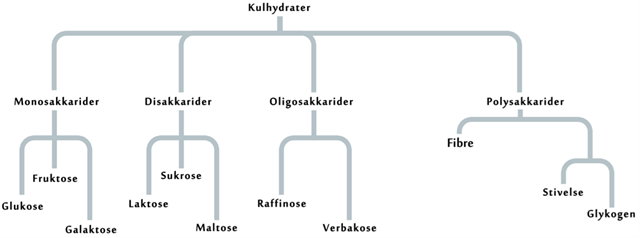
\includegraphics[width=0.8\textwidth]{figurs/carbs.png}
            \caption{Kulhydraterne inddeles i fire forskellige klasser afhængig af deres størrelse: monosakkarider, disakkarider, oligosakkarider og polysakkarider.}
            \label{fig:carbs}
        \end{figure}
        \begin{figure}
            \centering
            
\includegraphics[width=0.8\textwidth]{figurs/monosakarid.png}
            \caption{Monosakkarider}
            \label{fig:monosakkarider}
        \end{figure}
        \subsubsection**{Monosakkarider}
            De vigtigste monosakkarider i fødevarer og i organismen er glukose, fruktose og galaktose (figur \ref{fig:monosakkarider}); disse er alle hexoser. Fødevarer indeholder naturligt kun meget lidt af de tre monosakkarider (Se downloade tabel under eksammens mappe). Dog indeholder fx modne vindruer ca. 6,6 g fruktose og 6,8 g glukose pr. 100 g.
            I en vandig opløsning og i kropsvæskerne forekommer monosakkarider i både en lige kæde og i en ringform (figur \ref{fig:monosakkarider}) i forholdet 1:99. Det vil sige i en ligevægt, hvor 99 molekyler ud af 100 er på ringstruktur, og ét molekyle er på den lige form. Ringen dannes mellem C-atomet og iltatomet (O) i hhv. aldehyd- eller ketongruppen (figur \ref{fig:monosakkarider}). Monosakkariderne kan påvises og kvantitativt bestemmes vha. deres evne til at reagere med andre stoffer, der er betinget af indholdet af aldehyd eller ketongrupper. Især aldehydgruppen oxideres let til karboxylsyre. Den frie aldehydgruppe i glukose bevirker, at glukose kan reagere med protein. En kronisk forhøjet glukosekoncentration i blodet kan bevirke, at flere glukoseenheder bindes til proteiner, hvorved deres proteinstruktur og funktion ændres. Disse ændringer i proteinernes struktur ses hos nogle patienter med diabetes (sukkersyge).

            Monosakkarider kan også være pentoser, hvilket vil sige, de har fem kulstofatomer. I kroppen dannes pentoser primært ud fra hexosen glukose. Frie pentoser forekommer sjældent, men de er bestanddele af nukleinsyrerne i DNA (deoxyribonukleinsyre) i cellernes kerne (nucleus) og RNA (ribonukleinsyre). Pentoser findes desuden i ufordøjelige kulhydrater (kostfibre).


        \subsection**{Protein}
            Når man taler om at skulle have store guns så skal man have gains. Når man taler om gains taler man om både proteiner og kulhydrater. Men hvad er proteiner? Proteiner er et stort molekyle ligesom glucose. Proteiner er opbygget af aminosyre der findes 20 forskellige aminosyre som kan kombineres på utailige måder. Denne kæde af aminosyre kaldes også for et peptid. bindningerne mellem aminosyrerne kaldes for peptidbindinger. Læs mere om  peptidbindinger i afsnit \ref{fig:peptidbindinger}. Der findes 4 proteinstrukture
            \begin{itemize}
                \item Primærstruktur (1 - struktur)
                \item Sekundærstruktur (2 - struktur)
                \item Tertiærstruktur (3 - struktur)
                \item Kvartærstruktur (4 - struktur)
            \end{itemize}
            \textbf{Primærstruktur} er den struktur som er den simpleste.
            En normal kæde af aminosyre er primær, det der intificere at det er primærstruktur er at Den starter med \begin{math}NH_2\end{math} og slutter med en syregruppe \begin{math}COOH\end{math}.
            \textbf{Sekundærstruktur} er den stuktur som man kalder for Alpha helix og er den struktur som er foldet om sig selv som en spiral. Den Sekundærstruktur findes også som beta foldeblad. Beta foldebald er en slags siksak struktur. Der er også en beta vendning. Denne struktur binder de andre strukturer sammen.
            \textbf{Tertiærstruktur} er den rummelige opbygning af Beta foldebald, Beta vendning og Alpha helix. For at holde den rummelige opbygning sammen er der nogle svolvbroer. (cystein \begin{math}HS\end{math})
           \textbf{Kvartærstruktur} det er en samling af små proteiner det kunne være: Hemoplin, den består af 4 små proteiner. Altså protein kompleks som af flere mindre proteiner


\section*{Hvilke funktioner har de forskellige makromolekyler i en organisme?}
Makromolekyler spiller en række forskellige roller i en organisme, afhængig af deres type:
    \subsection**{Proteiner}
        Proteiner fungerer som kroppens arbejdsheste, udfører de fleste af de cellulære processer, der holder en organisme i live. Proteiner kan handle som enzymer, der katalyserer kemiske reaktioner; som strukturelle komponenter, der giver celler og væv form; som transportmolekyler, der bærer stoffer rundt i kroppen; og som antistoffer, der bekæmper infektioner.

    \subsection**{Nukleinsyrer}
        Nukleinsyrer, herunder DNA og RNA, er ansvarlige for lagring og transmission af genetisk information. DNA lagrer den genetiske information, der bestemmer organismens egenskaber, mens RNA bruges til at oversætte denne information til proteiner.
    
    \subsection**{Kulhydrater}
        Kulhydrater tjener primært som energikilde for celler. Enkle sukkerarter, såsom glukose, kan bruges direkte til energi, mens komplekse kulhydrater, som stivelse og cellulose, kan lagre energi eller give struktur til celler og væv.
    \subsection**{Lipider}
        Lipider er involveret i en række forskellige funktioner, herunder energilagring, isolering, celledeling (som en del af cellemembranen) og signalering (som hormoner). For eksempel lagrer triglycerider energi, fosfolipider danner cellemembraner, og steroider fungerer som signalstoffer.

    Hver type makromolekyle spiller forskellige roller, men de arbejder alle sammen for at støtte livets processer i en organisme.
\section*{Diskuter kostens betydning i forhold til sundhed. Inddrag øvelsen om kulhydrater i fødevarer}
    Kosten spiller en væsentlig rolle i forhold til sundhed. Her er nogle af de vigtige punkter, der understreger kostens betydning:

    Næringsstoffer: Den mad, vi spiser, forsyner vores krop med nødvendige næringsstoffer som proteiner, kulhydrater, fedt, vitaminer og mineraler. Disse næringsstoffer er nødvendige for kroppens forskellige funktioner, herunder energiproduktion, vævsvækst og reparation, og immunfunktion.

    Vægtkontrol: En afbalanceret kost hjælper med at vedligeholde en sund vægt. Overvægt og fedme, som ofte er resultatet af en usund kost, kan føre til forskellige sundhedsproblemer, herunder hjertesygdomme, type 2-diabetes og visse typer kræft.

    Sygdomsforebyggelse: En sund kost kan hjælpe med at forebygge visse sygdomme. For eksempel kan et kosthøjt i frugt og grønt, fuldkorn og magre proteiner hjælpe med at forebygge hjertesygdomme. En kost lav på sukker og mættet fedt kan hjælpe med at forebygge type 2-diabetes.

    Knoglesundhed: Indtagelse af nok calcium og D-vitamin i kosten er afgørende for knoglesundheden.

    Fordøjelsessystemets sundhed: En kost rig på fiber kan hjælpe med at forbedre fordøjelsessystemets sundhed ved at forebygge forstoppelse og reducere risikoen for visse sygdomme som tyktarmskræft.

    Mental sundhed: Nogle undersøgelser tyder på, at visse næringsstoffer som omega-3 fedtsyrer kan bidrage til mental sundhed ved at reducere symptomer på depression og angst.

    Selvom kosten er et centralt element i at opretholde en god sundhed, er det vigtigt at huske, at andre livsstilsfaktorer, som regelmæssig motion, tilstrækkelig søvn og undgåelse af tobak og overdreven alkohol, også er afgørende for vores overordnede velvære.
\section*{Mere info}
\begin{figure}[h]
    \centering
    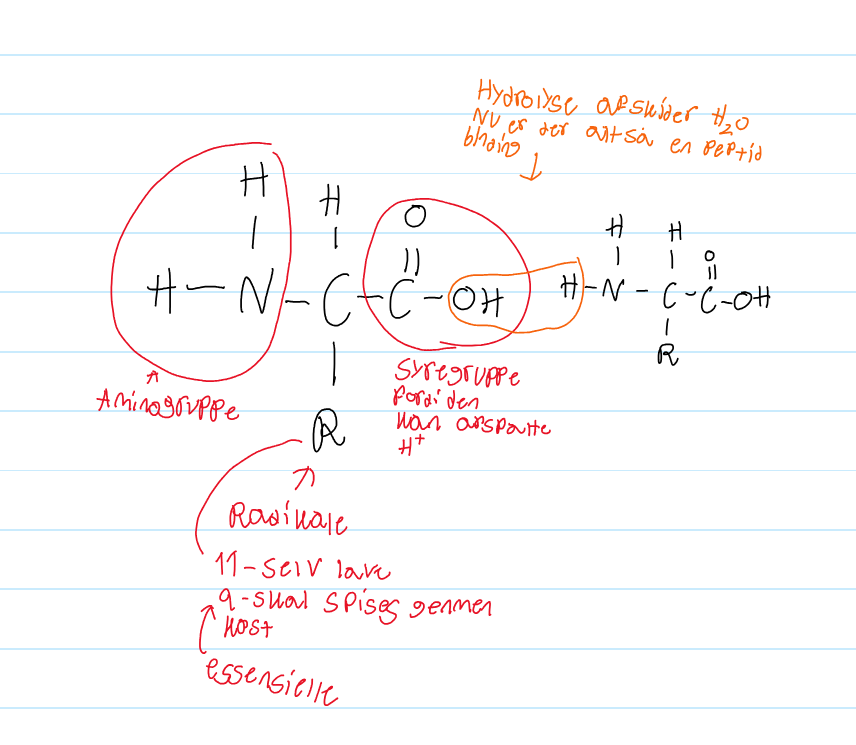
\includegraphics[width=0.8\textwidth]{figurs/peptidbindinger.png}
    \caption{Peptidbindinger}
    \label{fig:peptidbindinger}
\end{figure}